\documentclass[a4paper]{article}

%% Language and font encodings
\usepackage[english]{babel}
\usepackage[utf8x]{inputenc}
\usepackage[T1]{fontenc}

%% Sets page size and margins
\usepackage[a4paper,top=3cm,bottom=2cm,left=3cm,right=3cm,marginparwidth=1.75cm]{geometry}

%% Useful packages
\usepackage{amsmath}
\usepackage{graphicx}
\usepackage[colorinlistoftodos]{todonotes}
\usepackage[colorlinks=true, allcolors=blue]{hyperref}

\usepackage[authoryear]{natbib}

%% My definition
\newcommand{\toshi}{\textcolor{blue}}
\newcommand{\laurie}{\textcolor{red}}
\newcommand{\rishi}{\textcolor{green}}
\newcommand{\iago}{\textcolor{purple}}

\newcommand{\disp}{\displaystyle}

\usepackage{enumitem}
\usepackage{algorithm}
\usepackage{algorithmicx}
\usepackage{algpseudocode}

\usepackage{color}
\definecolor{darkgreen}{rgb}{0.0, 0.5, 0.0}
\definecolor{darkred}{rgb}{0.7, 0.11, 0.11}
\definecolor{darkblue}{rgb}{0,0,0.5}
\definecolor{shadecolor}{rgb}{1,1,0.95}
\definecolor{shade}{rgb}{1,1,0.95}
\definecolor{coilin}{rgb}{1,0,1}

\title{Is It You or Your Model Talking}
\author{Laurie Kell, Toshihide Kitakado, Rishi Sharma, ...}

\begin{document}
\maketitle
 
\section*{Outline}

\begin{itemize}
    \item The provision of fisheries management advice requires the assessment of stock status relative to reference points, the prediction of the response of a stock to management, and checking that predictions are consistent with reality (Holt pers com.)    
    \item Often when conducting a stock assessment multiple models with different structures and datasets, are used to explore uncertainty. This means that it is difficult to compare models using conventional metrics such as AIC. The use of metrics based on prediction skill allows different data components and model to be compared in order to explore data conflicts and potential model misspecification. %The accuracy and precision of predictions depend on the validity of the model, the information in the data, and how far ahead we wish to predict. 
    \item Retrospective analysis is commonly used to evaluate the stability of stock assessment estimates, however, stability can be at the expense of prediction skill, i.e. by using shrinkage. We therefore predict forward the retrospective analyses and then compare model predictions with historical estimates.The absence of retropective patterns, however, while reassuring is not sufficient alone as it is not possible to validate models based on model outputs. We therefore conduct model free hindcasts to compare observations with model estimates. 
    \item  We  compare SS, SS-ASPM, and Jabba assessments for Indian Ocean yellowfin tuna  using multiple metrics, make recommendations for benchmarking of stock assessments and discuss the consequences for MSE, i.e. weighting of OMs and developing OEMs.    
    %\item How to expand the hindcast to include a jackknife to estimate prediction residuals, and perform the hindcast by series.
\end{itemize}

\tableofcontents 

\newpage    
\begin{abstract}
    Evaluating how well the model fits data has been receiving much attention in fisheries science, both in terms of goodness-of-fit and retrospectively. This however merely tells us how well we can describe the past, yet little how well we can predict the future under alternative management actions. In this paper, we revisit the concepts behind hindcasting cross-validation (hcxval) as an important model-free validation tool for predictive modelling. Together with conventional residual diagnostics and retrospective analysis, we apply hcxval to three examples of alternative candidate models using the recent Indian Ocean yellowfin tuna assessment as a case study. 
    These models comprise the 2019 spatially structured reference model implemented in Stock Synthesis (ss-ref), a deterministic age-structured production model (ss-aspm) of ss-ref and a simplied spatially aggregated stochastic surplus production model implemented in the 'JABBA' package. To assess prediction skill, we computed the Mean-Absolute-Scaled-Error (MASE), which, unlike e.g. Aikaike's Information Criterion, enables to compare across different models fitted different data. The best MASE values (MASE < 1) were determined for ss-asem, which indicates that recruitment deviations in ss-ref were poorly estimated due to no or limited information in the 'noisy' length composition data. By contrast, the area effects retained in ss-aspm best explained its superior prediction skill compared to the spatially aggregated jabba model. We suggest that one-step ahead predictions are efficient for detecting overfitting and for model validation in general, but for future quota advice the forecast horizon should preferably at least match the assessment interval to ultimately increase confidence in the model-based scientific advice by stake holder and managers and policy makers.
\end{abstract}

\newpage
\section{Introduction}

In stock assessment most goodness of fit diagnostic are based on residuals obtained from fits to historical observations. To provide fisheries management advice, however, requires predicting the response of a stock to management and checking that the predictions are consistent with reality (pers. com. Sidney Holt). The accuracy and precision of predictions depend on the validity of the model, the information in the data, and how far ahead we wish to predict. Validation examines if a model should be modified or extended and is complementary to model selection and hypothesis testing. Model selection searches for the most suitable model within a family, whilst hypothesis testing examines if the model structure can be reduced.

Model validation is important in many fields, e.g. in energy and climate models, as it increases confidence in the outputs of a model and leads to an increase in trust amongst the public, stake and asset-holders and policy makers. For models to be valid they must satisfy four prerequisites \cite{hodges1992you}, the situation being modelled must be observable and measurable, it must be possible to collect sufficient data, exhibit constancy of structure in time, and exhibit constancy across variations in conditions not specified in the model. The first two prerequisites should be straight forward, but many stock assessments depend on fisheries dependent data rather than scientific observation. For example highly migratory stocks fished in areas beyond national jurisdiction (ABNJ). Prerequisite 3 ensures that the model has predictive skill for the same conditions under which the validation tests were conducted. Prerequisite 4 ensures that the model will still be valid for conditions that differ from those in the validation tests, i.e. can be used to set robust management advice. 

To explore the robustness of advice to uncertainty requires different model structures to be condition on alternative and potentially conflicting datasets. In such cases model selection criteria such as AIC, however, cannot be applied. The first prerequisite means it is not possible to validate a model, using derived quantities, such as SSB and F. The key concept in this case is prediction skill, defined as any measure of accuracy of a forecasted value to the actual (i.e. observed) value that is not known by the model \citep{glickman2000glossary}. Therefore  An alternative is to use model-free hindcasting, a form of crossvalidation where observations are compared to their predicted values.

To illustrate the utility of hindcasting we develop a case study based on bigeye and yellowfin tuna stocks in the Indian, Atlantic and Eastern Pacific Oceans, and four assessment methods, SS, SS-ASPM, Jabba-Select and Jabba. 

\section{Material and Methods}

\cite{kell2016xval} proposed a model-free hindcasting using crossvalidation where observations (e.g. CPUE) are compared to their predicted future values. The hindcasting algorithm is similar to that used in retrospective analysis \citep{hurtado2014looking}, which involves sequentially removing  observations from the terminal year (peels), fitting the model to the truncated series, and then comparing the difference between model estimates from the truncated time-series to those estimated using the full time series. In a model-free hindcast an additional step is included, i.e. projecting over the missing years and then cross-validating these forecasts against observations to assess the model’s prediction skill.

\subsection{Assessment Methods}

Case study based on Indian Ocean yellowfin tuna stocks and four assessment methods, SS, SS-ASPM, Jabba-Select and Jabba. 

\begin{verbatim}
There has been a recent trend in stock assessment to use integrated analysis that combines several sources of data into a single model by a joint likelihood for the observed data (Doubleday, 1976, Fournier and Archibald, 1982, Maunder and Punt, 2013).  Datasets include records of catches and landings, indices of abundance based on catch per unit (CPUE) and from research surveys, and the length classes and/or ages compositions based on samples. A commonly used integrated assessment method is Stock Synthesis (Methot and Wetzel, 2013) that can be configured in multiple ways e.g. SSS and ASPM.

Alternatives are biomass dynamic models based on a surplus production function that requires the estimation or fixing of fewer parameters, since many parameters required in integrated assessments are difficult to estimate in practice (e.g. Lee et al.). Once such example is JABBA an open source package that presents a unifying, flexible framework for biomass dynamic modelling, runs quickly, and generates https://www.overleaf.com/project/5ca9fed01e2a625dbaeae31freproducible stock status estimates.

A problem is how to compare these different models


\begin{description}
\item{SS} 
Stock Synthesis (Methot and Wetzel 2013; SS) is widely used to perform integrated assessments for fish stocks in the United States and throughout the world. While Stock Synthesis is typically applied in data-rich circumstances, its use in data-moderate stock assessments (where catch time series and abundance indices are available, and catch composition data is limited or absent) has significantly increased in recent years. The uptake of Stock Synthesis for integrated data-moderate stock assessments has occurred especially in assessments developed for Regional Fishery Management Organizations (RFMOs). Various stocks of billfish and pelagic sharks that were historically assessed using Surplus Production Models and Virtual Population Analysis (VPA) are now moving towards full implementation in Stock Synthesis as additional data become available (e.g. Courtney et al. 2017; Schirripa 2019). Similarly, there has been a recent increase in Stock Synthesis benchmark assessment in Europe in place of the conventionally used VPA with extended survivor analysis (XSA) in the region (Max Refs). The visualization of model outputs and implementation of diagnostics for Stock Synthesis is facilitated by the availability of a comprehensive collection of R functions (r4ss; https://github.com/r4ss).

\item{ASPM} 
Maunder and Piner (2015) proposed the ASPM age-structured production model (ASPM) as a diagnostic of process dynamics. This diagnostic evaluates whether the observed catches alone (taken out of approximately the correct ages) can explain trends in the index of abundance. On the one hand, Maunder and Piner (2015) suggest that if the ASPM is able to fit well to the indices of abundance that have good contrast (i.e. those that have declining as well as increasing trends), the production function likely exists, and the indices will provide information about absolute abundance. On the other hand, the authors suggest that if there is not a good fit to the indices, then the catch data alone cannot explain the trajectories depicted in the indices of relative abundance. This can have several causes: (i) the stock is recruitment-driven; (ii) the stock has not yet declined to the point at which catch is a major factor influencing abundance; (iii) the base-case model is incorrect; or (iv) the indices of relative abundance are not proportional to abundance. Alternatively, failure in the ASPM may indicate a system that is not well organized (e.g., stock structures or data are incorrect) so that a real fishing signal is lost or where unknown environmental drivers control population abundance. The ASPM was shown via simulation analyses to be the only tested diagnostic capable of detecting misspecification of the key systems-modeled processes that control the shape of the production function (Carvalho et al., 2017).
\item{Jabba}
This study presents a new, open-source modelling software entitled ‘Just Another Bayesian Biomass Assessment’ (JABBA). JABBA can be used for biomass dynamic stock assessment applications, and has emerged from the development of a Bayesian State-Space Surplus Production Model framework, already applied in stock assessments of sharks, tuna, and billfishes around the world. JABBA presents a unifying, flexible framework for biomass dynamic modelling, runs quickly, and generates reproducible stock status estimates and diagnostic tools. Specific emphasis has been placed on flexibility for specifying alternative scenarios, achieving high stability and improved convergence rates. Default JABBA features include: 1) an integrated state-space tool for averaging and automatically fitting multiple catch per unit effort (CPUE) time series; 2) data-weighting through estimation of additional observation variance for individual or grouped CPUE; 3) selection of Fox, Schaefer, or Pella-Tomlinson production functions; 4) options to fix or estimate process and observation variance components; 5) model diagnostic tools; 6) future projections for alternative catch regimes; and 7) a suite of inbuilt graphics illustrating model fit diagnostics and stock status results. As a case study, JABBA is applied to the 2017 assessment input data for South Atlantic swordfish (Xiphias gladius). We envision that JABBA will become a widely used, open-source stock assessment tool, readily improved and modified by the global scientific community.
\end{description}\end{verbatim}

\subsection{Procedure}

\subsubsection{Residuals}

%Analysis of residuals is a common way to determine a model’s goodness-of-fit \citep{Cox1968general}. For example non-random patterns in the residuals may indicate model misspecification, serial correlation in sampling/observation error, or that heteroscedasticity is present. Various statistics exist to evaluate the residuals for desirable properties and nonparametric tests for randomness in a time-series include: the runs test, the sign test, the runs up and down test, the Mann-Kendall test, and Bartel’s rank test.
If the process of interest shows only random variation, the data points will be randomly distributed around the median. Random meaning that we cannot know if the next data point will fall above or below the median, but that the probability of each event is 50\%, and that the data points are independent. Independence means that the position of one data point does not influence the position of the next data point, that is, data are not auto-correlated. If the process shifts, these conditions are no longer true and patterns of non-random variation may be detected by statistical tests. 
Non-random variation may present itself in several ways. If the process centre is shifting due to improvement or degradation we may observe unusually long runs of consecutive data points on the same side of the median or that the graph crosses the median unusually few times. The length of the longest run and the number of crossings in a random process are predictable within limits and depend on the total number of data points in the run chart \citep{anhoj2015diagnostic}.
A shift signal is present if any run of consecutive data points on the same side of the median is longer than the prediction limit, round(log2(n) + 3). Data points that fall on the median do not count, they do neither break nor contribute to the run \cite{schilling2012surprising}. A crossings signal is present if the number of times the graph crosses the median is smaller than the prediction limit, qbinom(0.05, n - 1, 0.5) \citep{chen2010impacts}. n is the number of useful data points, that is, data points that do not fall on the median. The shift and the crossings signals are based on a false positive signal rate around 5\% and have proven useful in practice.

\subsubsection{Retrospective}

%In a retrospective analysis a model is fitted to increasing periods of data to identify systematic inconsistencies \citep{Mohn1999retrospective}.

%Retrospective analysis is a hindcasting approach that involves sequentially removing observations from the terminal year (peels), fitting the model to the truncated series and then comparing the relative difference between model estimates from full time series with the truncated time-series. Retrospective analysis focuses on the bias and accuracy of modeled quantities. 

The most commonly used statistic to assess the strength of patterns is Mohn’s $\rho$ a measure of relative error

\begin{equation}\rho = \overline{ \left[ \frac{X_{Y-p,ref}-X_{Y-y,ref}}{X_{Y-y,ref}} \right]}\end{equation}

where $X$ is the quantity for which Mohn’s $\rho$ is being calculated, $Y$ the final year of the simulation, $y$ the last year of a given “peel” $p$, and $ref$ the reference peel, i.e. the most recent assessment.

The difference between the reference ($X{ref}$) the alternative peeled model ($X{p}$) is calculated using the relative error 

\begin{equation} RE=\frac{X_{p}-X_{ref}}{X_{ref}} \end{equation}
    
There are problems with the use of $RE$, since for reference model estimates which are low relative to the alternative model, i.e. $X_{ref} < X_{p}$, there is no upper limit, while for $X_{ref} > X_{p}$ the error cannot exceed 1.0. Therefore the chosen metric puts a heavier penalty on negative than on positive errors, i.e. historical underestimates. This means that when comparing models estimates, those that are low will be preferred. This problem can be overcome by using the logarithm of the ratio instead i.e. $log\frac{X_{p}}{X_{ref}}$, which also leads to better statistical properties.

While it is fairly straightforward to compare the  statistic among alternative model runs, the decisions of whether the Mohn’s $\rho$ statistic of the ‘best’ model is acceptable or not can be to some extent subjective. To address this, a “rule of thumb” was proposed by \cite{hurtado2014}, suggesting values of Mohn’s $\rho$ that fall outside the range (-0.15 to 0.20) can be interpreted as an indication of an undesirable retrospective pattern for e.g. longer lived species.






\subsubsection{Retrospective with Projection}
#When conducting projections to provide managers with advice,such as a total allowable catch (TAC), the short term is of primary importance as usually the immediate consequences of management advice is a major concern of stakeholders \citep{fricker2013three}. Therefore we also conduct projections for 3 years as part of the retrospective analysis.#


\subsection{Hindcast}

%When inspecting residuals there is a danger of hypothesis fishing and if multiple true hypotheses are tested it is likely that some of them will be rejected. Therefore it is valuable to reserve part of the data for validation, so that a pattern’s significance is not tested on the same data set which suggested the pattern.


\begin{algorithm}[!ht]
\begin{algorithmic}[1]
\State $t=0$
\State initialize $P_{t}$
\State evaluate structures in $P_{t}$
\While {termination condition not satisfied}
\State $t=t+1$
\State select reproduction $C_{t}$ from $P_{t-1}$
\State recombine and mutate structures in $C_{t}$

forming $C'_{t}$
\State evaluate structures in $C'_{t}$
\State select each individual for $P_{t}$ from $C'_{t}$ 

or $P_{t-1}$
\EndWhile
\caption{Genetic algorithm \cite{FogelDavidB2009}}
\label{genetic-algorithm}
\end{algorithmic}
\end{algorithm}

\subsubsection{Summary Metrics}

%A well-fitting model results in predicted values close to the reference values, i.e. if $Y_t$ is the variable of interest at time $t$ and ${\hat{Y}_t}$ is it's predicted value then the prediction error is $e_t = Y_t - \hat{Y}_t$ and should be small. The accuracy of the predictions can be assessed by various measures. One example is the Mean Absolute Error (MAE), which is the mean of the absolute errors and measures how big of an error the forecast will generate on average.

\begin{equation} 
{MAE} =\frac{\sum_{i=1}^{n}\left|e_{i}\right|}{n}
\end{equation} 
 
A problem with the MAE is that the relative size of the error is not always obvious. Sometimes it is hard to tell a big error from a small error. To deal with this problem, the MAPE can be calculated instead, i.e. MAE as a percentage, this allows forecasts of different series in different scales to be compared.

\begin{equation} 
{MAPE = \frac{1}{T} \sum_{t=1}^T 100\, \left|\frac{e_t}{Y_t}\right|} 
\end{equation}

Both MAE and MAPE are based on the mean absolute error and so may understate the impact of big, but infrequent, errors.  To adjust for large rare errors the Root Mean Square Error (RMSE) squares the errors before calculating their mean i.e.
     
\begin{equation} 
{E^{\prime} = \sqrt{\frac{1}{T} \sum_{t=1}^T e_t^2}} 
(better to say RMSE like other measures for consistency?)
\end{equation}

This is the square root of the variance of the residuals (strictly if the mean of the residuals is 0 and practically if that is nearly 0) and indicates how close predicted values are close to the observations. As the square root of a variance it can also be interpreted as the standard deviation of the unexplained variance, and so lower values indicate better fits. Although RMSE,is commonly used when simulation testing assessment models \citep[e.g.][]{horbowy2011comparison} as described above it does not describe average error alone, is sensitive to outliers, favours forecasts that avoid large deviations from the mean, and cannot be used to compare across series.

The best statistical measure to use depends on the objectives of the analysis and using more than one measure can be helpful in providing insight into the nature of observation and process error structures. For example the correlation ($\rho$) between $Y_y$ and $\hat{Y_y}$ is not affected by the amplitude of the variations, is insensitive to biases and errors in variance, and can be used to compare across series.

$E^{\prime 2}$ and $\rho$ are related by the cosine rule i.e

\begin{equation} 
{E^{\prime 2} = \sigma_o^2 + \sigma_f^2 - 2\sigma_o\sigma_f\rho},
\end{equation}

where the reference set ($o$) are the observations ($Y_t$) not included in the retrospective assessment and the values (f) are their estimates ${\hat{Y}_t}$. This means that $E^\prime$, $\rho$ and $\sigma_f$ can be summarised simultaneously  \citep{taylor2001summarizing}. Taylor diagrams therefore provide a concise statistical summary of how well patterns match each other and are therefore especially useful for evaluating multiple aspects or in gauging the relative skill of different models \citep{griggs2002climate}. We can also compare RMSE and MAE to determine whether the forecast contains large but infrequent errors. The larger the difference between RMSE and MAE the more inconsistent the error size.

A more robust and easier to interpret statistic for evaluating prediction skill is the Mean Absolute Scaled Error (MASE) \citep{hyndman2006another}. MASE evaluates a model’s prediction skill relative to a na\ddot{i}ve baseline prediction. A prediction is said to have skill if it improves the model forecast compared to the baseline. A widely used baseline forecast for time series is the persistence algorithm that simply takes the value at the previous time step to predict the expected outcome at the next time step as a na\ddot{i}ve in-sample prediction, i.e. tomorrow will the same as today 

The MASE score scales the mean absolute error of the forecasts by the mean absolute error of a na\ddot{i}ve in-sample prediction, such that:

For a series of $T$ observations and predictions

\begin{equation} 
{MASE=\frac{\frac{1}{T} \sum_{t=1}^{T} \left|e_{t}\right|}
{\frac{1}{T-1} \sum_{t=2}^{T} \left|Y_{t+1}-Y_{t}\right|}}
\end{equation}

The MASE has the desirable properties of scale invariance, predictable behaviour, symmetry, interpretability and asymptotic normality. The scale invariance of MAPE and MASE allows us to compare forecasts across data sets with different scales, while MAE does not have such a feature. When it comes to the predictable behavior, percentage forecast accuracy measures rely on division of $y_{t}$, skewing the distribution of the MAPE for values of $y_{t}$ near or equal to 0. This is especially problematic for data sets whose scales do not have a meaningful 0, such as temperature in Celsius or Fahrenheit, and for intermittent demand data sets, where $y_{t}=0$  occurs frequently. With respect to symmetry, the MASE penalises positive and negative forecast errors equally, and penalises errors in large forecasts and small forecasts equally. The MASE can also be easily interpreted, as values greater than one indicate that in-sample one-step forecasts from the na\ddot{i}ve method perform better than the forecast values under consideration, in other words model forecasts are worse than a random walk. Conversely, a MASE score of 0.5 indicates that the model forecasts twice as accurate as a na\ddot{i}ve baseline prediction; thus the model has prediction skill.

[I now realized you used \iffalse.... I re-do...] 

\iffalse
If $Y_t$ is a variable of interest at time $t$ and \eqn{\hat{Y}_t} is it's predicted value then the prediction error is given by $e_t = Y_t - \hat{Y}_t$. For a series of $T$ observations and predictions The accuracy of the predictions can be compared to the actual value by calculating various measures, such as as the Mean Absolute Error (MAE), which is the mean of the absolute errors and tells us how big of an error we can expect from the forecast on average. \\

\eqn{MAE=\frac{\left|e_t\right|}{T}} \\

A problem with the MAE is that the relative size of the error is not always obvious. Sometimes it is hard to tell a big error from a small error. To deal with this problem, we can compute the MAPE instead, i.e. MAE as a percentage, this allows forecasts of different series in different scales to be compared.\\

\eqn{MAPE = \frac{1}{T} \sum_{t=1}^T 100\, \left|\frac{e_t}{Y_t}\right|}\\

Both MAE and MAPE are based on the mean error and so may understate the impact of big, but infrequent, errors. If we focus too much on the mean, we will be caught off guard by the infrequent big error. To adjust for large rare errors, we calculate the Root Mean Square Error (RMSE). By squaring the errors before we calculate their mean and then taking the square root of the mean, we arrive at a measure of the size of the error that gives more weight to the large but infrequent errors than the mean.\\

\eqn{RMSE = \sqrt{\frac{1}{T} \sum_{t=1}^T e_t^2}} \\

We can also compare RMSE and MAE to determine whether the forecast contains large but infrequent errors. The larger the difference between RMSE and MAE the more inconsistent the error size.
 
Another measure is the Mean Absolute Scaled Error (MASE) \\

\eqn{MASE={\frac {\sum _{t=1}^{T}\left|e_{t}\right|}{{\frac {T}{T-1}}\sum _{t=1}^{T}\left|Y_{t+1}-Y_{t}\right|}}} \\

Which has the desirable properties of scale invariance, predictable behaviour, symmetry, interpretability and asymptotic normality
 
The mean absolute scaled error is independent of the scale of the data, so can be used to compare forecasts across data sets with different scales. Behaviour is predictable as $y_{t}\rightarrow 0$] Percentage forecast accuracy measures such as the Mean absolute percentage error (MAPE) rely on division of $y_{t}$, skewing the distribution of the MAPE for values of $y_{t}$ near or equal to 0. This is especially problematic for data sets whose scales do not have a meaningful 0, such as temperature in Celsius or Fahrenheit, and for intermittent demand data sets, where $y_{t}=0$  occurs frequently.

Symmetry since The mean absolute scaled error penalises positive and negative forecast errors equally, and penalises errors in large forecasts and small forecasts equally. In contrast, the MAPE  fail both of these criteria. The mean absolute scaled error can be easily interpreted, as values greater than one indicate that in-sample one-step forecasts from the naïve method perform better than the forecast values under consideration.The Diebold-Mariano test for one-step forecasts is used to test the statistical significance of the difference between two sets of forecasts. To perform hypothesis testing with the Diebold-Mariano test statistic, it is desirable for $DM ∼ N ( 0 , 1 )$ $DM\sim N(0,1)$ , where $DM$ is the value of the test statistic. The DM statistic for the MASE has been empirically shown to approximate this distribution, while the mean relative absolute error (MRAE), MAPE and sMAPE do not.
 
Another measure is Theil's $U$\\
  
\eqn{U= \sqrt{\frac{1}{T}\\
     \sum_{t=1}^{T-1} \left(\frac{e_{t+1}}{Y_t}\right)^2
     \cdot \left[
    \frac{1}{T} \sum_{t=1}^{T-1} 
        \left(\frac{Y_{t+1} - Y_t}{Y_t}\right)^2 \right]^{-1}}}

The more accurate the forecasts, the lower the value of Theil's $U$,   which has a minimum of 0. This measure can be interpreted as the ratio of the RMSE of the proposed forecasting model to the RMSE of  a na\"ive model which simply predicts $Y_{t+1} = Y_t$ for all $t$. The na\"ive model yields $U = 1$; values less than 1 indicate an  improvement relative to this benchmark and values greater than 1 a deterioration.

Altough the methods have their limitations, they are simple tools for evaluating forecast accuracy that can be used without knowing anything about the forecast except the past values of a forecast.

Just because a forecast has been accurate in the past, however, does not mean it will be accurate in the future. Over fitting may make the forecast less accurate and there is always the possibility of an event occurring that the model cannot anticipate, a black swan event. When this happens, you don’t know how big the error will be. Errors associated with these events are not typical errors, which is what the statistics above try to measure. So, while forecast accuracy can tell us a lot about the past, remember these limitations when using forecasts to predict the future.

\fi

\section{Results}

Figure~\ref{fig:map} shows the stock distribution shows the stock structure assumed in the SS assessments.

The first step was to conduct a retrospective analysis and the estimates of stick biomass (SSB for ASPM and SS, and biomass for JABBA) and F (instantaneous for ASPM and SS, and rate for JABBA) are shown in Figure~\ref{fig:retro}. The terminal estimates were then project forward for three years assuming the reported catches and the estimated recruitment from the model with all years included  (Figure~\ref{fig:predictions}). ASPM "predicted" values are close to those of the assessment that includes all years. For SS, however, there is a large overestimation of future biomass, and a underestimate of F . For JABBA the strongest retrospective pattern is seen in F, which is underestimated in the predictions.

The residuals from the model fits are shown in Figure~\ref{fig:runs}, the backgroud indicates whether they passed (green) or failed (red) the runs tests. 

The results from the model-free  Hindcast with one year ahead predictions are shown in Figure~\ref{fig:hy1} and from the three year ahead predictions in Figure~\ref{fig:hy3}.

Figure~\ref{fig:runshat} shoes the predictions residuals, and the fits are summarised in Figures~\ref{fig:td} and Figure~\ref{fig:tdhat} in the form of Taylor diagrams

\subsection*{Summary}

\begin{description}
    \item{Retrospective analysis and projections for F/FMSY and B/BMSY} show that
    \begin{itemize}
        \item SS projections and hence advice is based upon SS is unreliable.
        \item Jabba advice is problematic as it appears that even if F<FMSY the stock will decline below BMSY
        \item ASPM appears consistent
        \item It therefore appears that the length compositions just add noise, and that area effects are important
        \item However these is no objective way to choose an assessment based on retrospective analysis as the best model would always be B/MSY = 1 
        \end{itemize}
    \item{Model-free cross-validation} confirms the relative performance of the models
    \begin{itemize}
        \item ASPM performs best
        \item Survey 2 performs poorly across all models
   \end{itemize}
   \item{Make case for why we need MASE and why this new methodology is important}
    \begin{itemize}
        \item Tabulate Metrics
        \item Compare MASE to other measures and use Taylor Diagrams to explain differences
   \end{itemize}

\end{description}

\section{Discussion}

\begin{verbatim}
I was thinking about running a jackknife to estimate the prediction residuals, but a problem is the serial correlations in the observations. So I think the one-step-ahead is a good procedure as it is pragmatic, since we are checking whether the next step will trip us up.

Apparently in the ICES benchmark assessments the main check is the retrospective analysis, however, if you used strong shrinkage, i.e. made current F and recruitment an average of recent values then there would be no retrospective pattern, But! when you projected the estimates would be crazy. Thats what the projections are important.

I was also thinking about removing the all indices 1 year-at-time together and doing it index by index.

Doing it all together is a good 1st step as it shows the transition from retrospective analysis of F&SSB to model free hindcast. But index by index allows us to see the impact of each index, which is important if we want to work out how to extend/modify the model.
I guess if we look at  model residuals we may say all the models were equally good, however, if we perform a 1,3, step ahead predictions we show that in fact SS is just modelling noise and Jabba by throwing everything into process error has little prediction skill, so we should choose ASPM an intermediate model, add area effects to Jabba.

te model should fit the trends in the abundance indices as well as possible,

Whitten, A.R., Punt, A.E., Taylor, B.L., 2013. Pink ling (Genypterus blacodes) stock
assessment based on data up to 2011. In: Tuck, G.N. (Ed.), Stock Assessment for
the Southern and Eastern Scalefish Fishery: 2013 Part X. Australian Fisheries
Management Authority and CSIRO Marine and Atmospheric Research, Hobart
(in press).


When inspecting prediction residuals, or other residuals, one scans for a large number of possible patterns, e.g. bias, drift, skewness, heavy tails, correlation with states
or driving inputs, and heteroscedasticity. One should avoid the dangers of hypothesis
fishing and recall that if multiple true hypotheses are tested, it is likely that some of
them are rejected. It is rarely possible to conceive a list of tests on the residuals before
seeing them, which means that the hypotheses we are testing, implicitly or explicitly,
are not proposed independently of data. This is not in agreement with the principles
of statistics; this is a well-known problem of post-hoc analysis. For that reason [and
several others, Wasserstein and Lazar (2016)] the ubiquitous significance level of 5%
should not be used uncritically. Similarly, it is recommendable to follow the general
advice of reserving part of the data for validation, so that a pattern’s significance is
not tested on the same data set which suggested the pattern.

A strong retrospective pattern is a problem with historical fits, which could be improved using shinkage, or even using a model with no prediction skill, i.e. simply saying that biomass = 1. So getting rid of a retrospective pattern is not necessarily fixing the problem. Neither can you validate a model using retrospective analysis. You need to do this by comparing fits to observations. So while the absence of retrospective patterns is nice, as it gives you 1 less thing to worry about it isnt sufficient.
 A MASE >1 means that a random walk is better than your model, i.e. you need a new model! This is probably because there are some processes that are not being modelled correctly or else the dataseries with MASE>1 do not contain information on stock abundance or are in conflict with those where MASE<1. Therefore you need to extend or revisit your model structure. MASE can be used to compare across models unlike AIC, so can still be used in this process to compare new models and datasets. For example in a paper we are drafting for Indian Ocean yellowfin we ran SS with area/quarter effects, ASPM-SS and JABBA, The best MASE values were seen for ASPM, this was because the length comps only added noise, and area effects were important but were not included in JABBA. In all  models the CPUE not in the main area of the fishery had MASE>1 and so was probbaly only add noise and should be excluded. So MASE allows models to be compared and the impact of datasets to be compared. Also by looking at predictions we are avoiding overfitting which could result in a retrospective pattern or poor prediction skill 
\\end{verbatim}
\section{Conclusions}


Primary objectives were:
\begin{enumerate}
    \item In fisheries unlike other fields we try to account for the past but not for the future. Here we propose a way to assess model predictive performance and to account for alternative models within a common diagnostic framework.  
    \item Unifying platform for evaluating across models
    \item Advantage of MASE : What are the new properties of this stat
\end{enumerate}


\bibliography{main.bib}
\bibliographystyle{apalike}

\section{Tables}

\section{Figures}

\begin{figure*}[htbp]
\centering
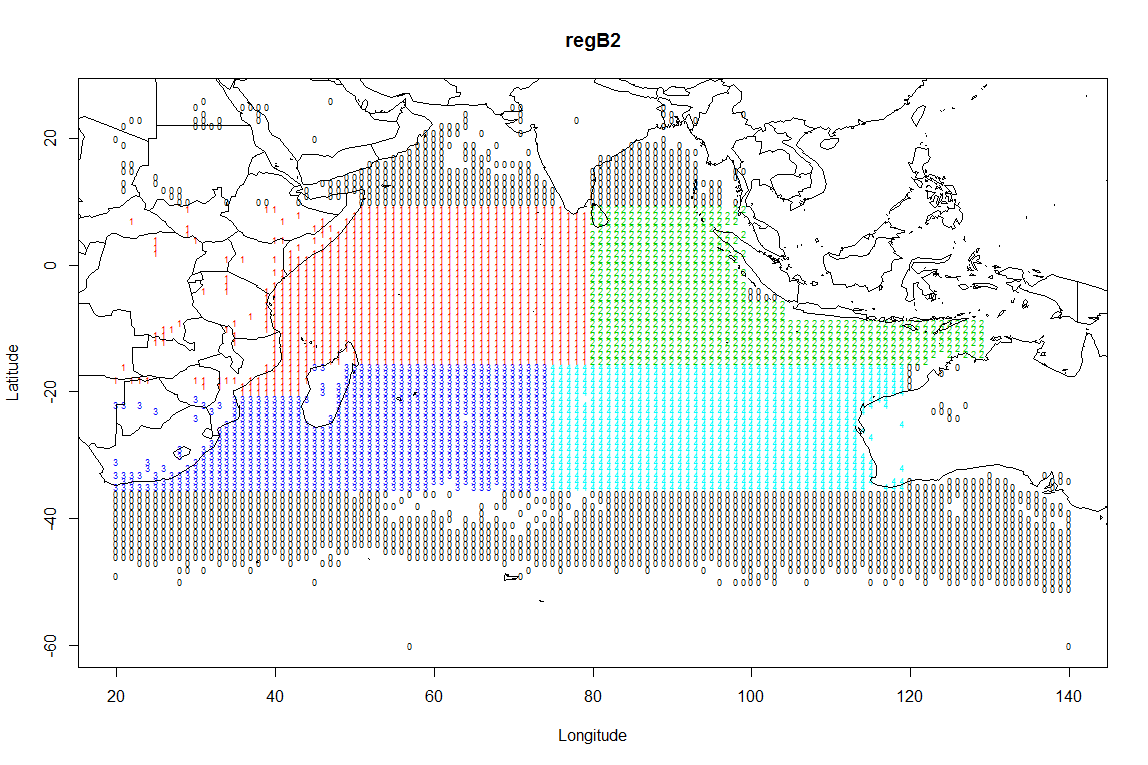
\includegraphics[width=6in]{map.png}
\caption{Stock distribution.}
\label{fig:map}
\end{figure*}

\begin{figure*}[htbp]
\centering
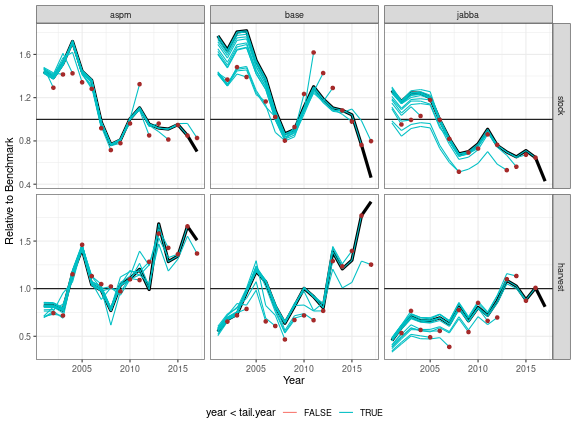
\includegraphics[width=6in]{final-retro-1.png}
\caption{Retrospective analysis for the three models, points indicate the terminal years, and the think line the assessment using all the data.}
\label{fig:retro}
\end{figure*}

\begin{figure*}[htbp]
\centering
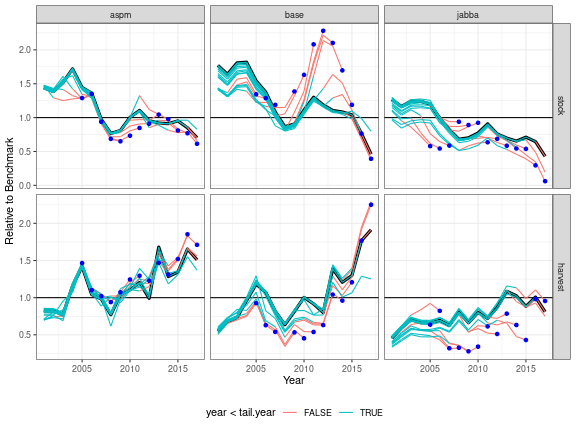
\includegraphics[width=6in]{final-retro3-1.png}
\caption{Retrospective analysis with three year predictions for the three models, points indicate the terminal years, and the think line the assessment using all the data.}
\label{fig:predictions}
\end{figure*}


\begin{figure*}[htbp]
\centering
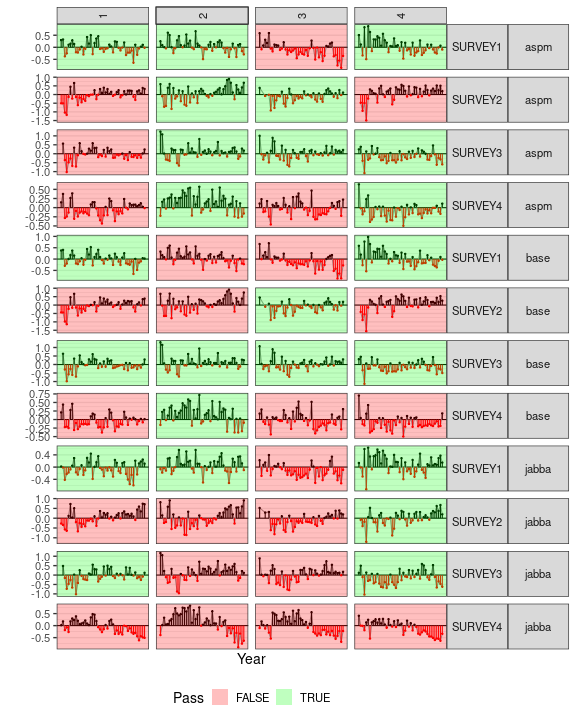
\includegraphics[width=6in]{final-cpue-residual-runs-1.png}
\caption{Residual runs tests for fits to the three models; green background indicates series where runs tests are passed.}
\label{fig:runs}
\end{figure*}

\begin{figure*}[htbp]
\centering
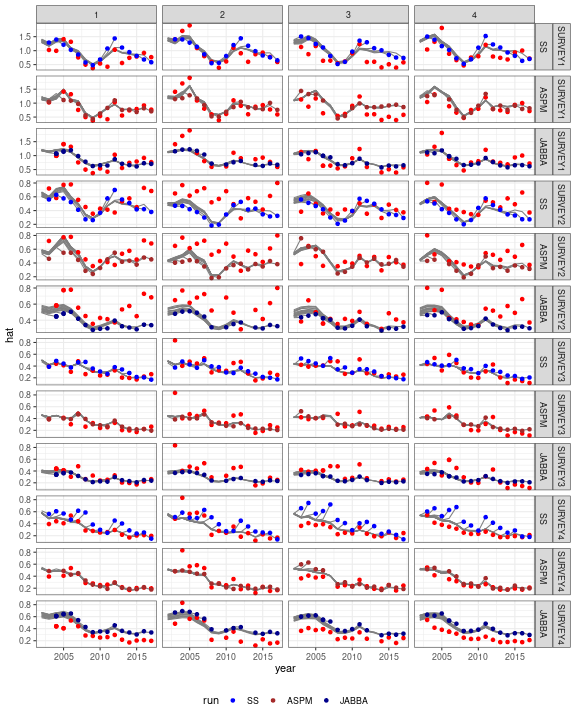
\includegraphics[width=6in]{final-hy-plot-1.png}
\caption{Hindcast with one year ahead predictions, red dots are the observed CPUE values and lines are the fits with terminal hincast year indicated by a point.}
\label{fig:hy1}
\end{figure*}

\begin{figure*}[htbp]
\centering
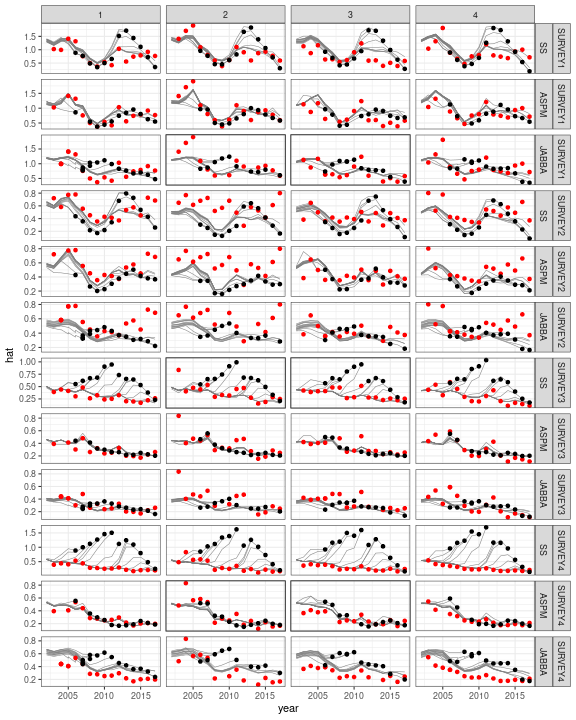
\includegraphics[width=6in]{final-hy3-plot-1.png}
\caption{Hindcast with three year ahead predictions, red dots are the observed CPUE values and lines are the fits with terminal hincast year indicated by a point.}
\label{fig:hy3}
\end{figure*}


\begin{figure*}[htbp]
\centering
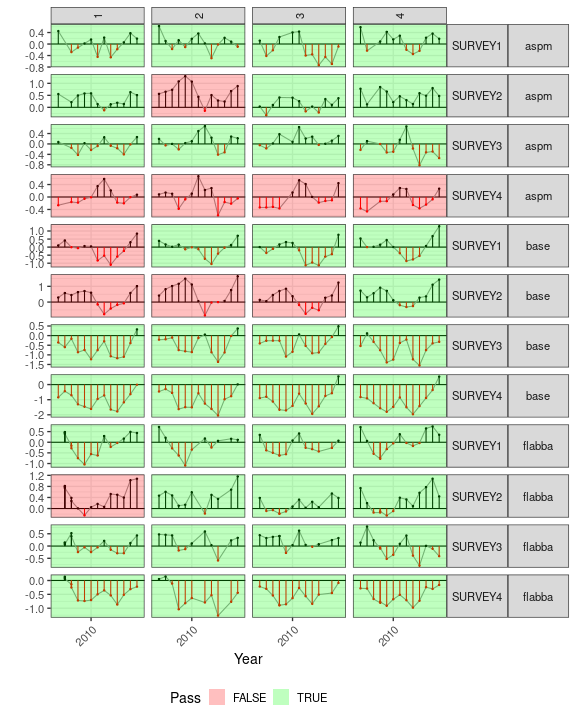
\includegraphics[width=6in]{final-cpue-prediction-runs-1.png}
\caption{Runs tests for one step ahead residuals.}
\label{fig:runshat}
\end{figure*}


\begin{figure*}[htbp]
\centering
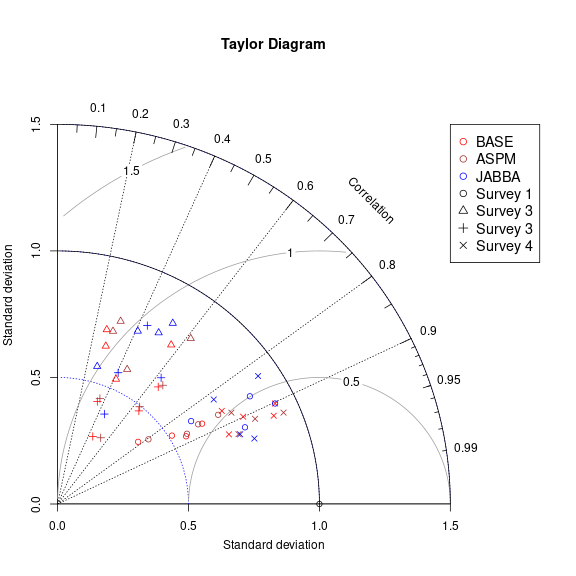
\includegraphics[width=6in]{final-taylor-residuals-1.png}
\caption{Taylor diagram for fits to CPUE summarising the similarity between the observed time series of CPUEs and the predicted relative stock abundance. Each point quantifies how closely predictions match observations, the angle indicates the correlation, the centred root-mean-square error difference between the predicted and observed patterns is proportional to the distance to the point on the x and the contours around this point indicate the RMSE values; the standard deviations of the predictions are proportional to the radial distance from the origin, scaled so the observed pattern has a value of 1. The open circle corresponds to a series which is identical to the reference series. The colours correspond to the model and shape to the survey.)}
\label{fig:td}
\end{figure*}

\begin{figure*}[htbp]
\centering
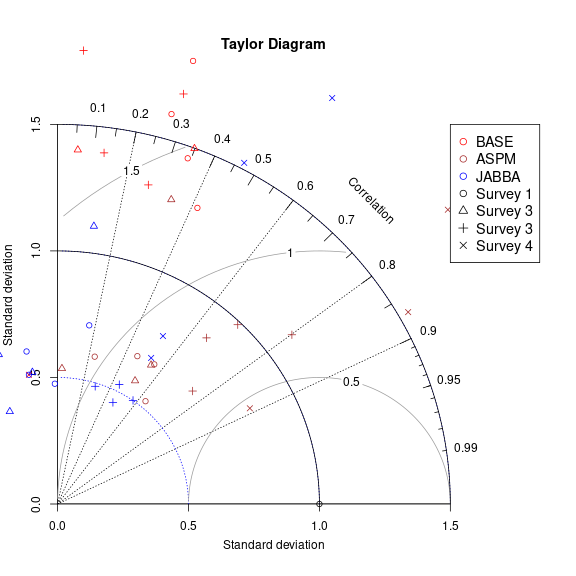
\includegraphics[width=6in]{final-taylor-hy-1.png}
\caption{Taylor diagram for 3 year ahead predictions, summarising the similarity between the observed time series of CPUEs and the predicted relative stock abundance. Each point quantifies how closely predictions match observations, the angle indicates the correlation, the centred root-mean-square error difference between the predicted and observed patterns is proportional to the distance to the point on the x and the contours around this point indicate the RMSE values; the standard deviations of the predictions are proportional to the radial distance from the origin, scaled so the observed pattern has a value of 1. The open circle corresponds to a series which is identical to the reference series. The colours correspond to the model and shape to the survey.}
\label{fig:tdhat}
\end{figure*}



\end{document}
